% Copyright (c) 2026 Pablo Suárez-Serrato. All rights reserved.
% Released under the GNU Affero General Public License v3.0 (AGPLv3) for non-commercial use;
% see LICENSE.md for details.
% This project is licensed under non-commercial use. If you wish to use this software in a
% commercial product, service, or enterprise environment, please contact the developer to purchase
% a commercial license or negotiate royalty terms.
% Authors: Pablo Suárez-Serrato (November 2026).
\pdfminorversion=7
\documentclass[10pt]{article}
\usepackage[margin=0.85in]{geometry}
\usepackage[T1]{fontenc}
\usepackage[utf8]{inputenc}
\usepackage{lmodern}
\usepackage{amsmath,amssymb,amsthm}
\usepackage{booktabs}
\usepackage{tabularx}
\usepackage{enumitem}
\usepackage{xcolor}
\usepackage{listings}
\usepackage{graphicx}
\usepackage{tikz}
\definecolor{bpgreen}{HTML}{1CAC78}
\definecolor{bpdef}{HTML}{B0ECA3}
\definecolor{bpblue}{HTML}{1F5FD6}
\usetikzlibrary{arrows.meta,positioning,shapes.geometric}
\usepackage[colorlinks=true,linkcolor=blue!50!black,citecolor=blue!50!black,urlcolor=blue!50!black]{hyperref}

\graphicspath{{./}{report/}}

\setlist{itemsep=1.5pt,topsep=3pt}
\emergencystretch=3em
\let\origus\_
\renewcommand{\_}{\origus\allowbreak}

\newtheorem{theorem}{Theorem}
\newtheorem{corollary}[theorem]{Corollary}
\newcommand{\R}{\mathbb{R}}
\newcommand{\Z}{\mathbb{Z}}
\newcommand{\N}{\mathbb{N}}
\newcommand{\code}[1]{\texttt{#1}}
\newcommand{\Crit}{\mathrm{Crit}}

% ---- Repository & Audit Metrics (report_tool.py metrics + independent audit) ----
\newcommand{\LeanToolchain}{leanprover/lean4:v4.36.0}
\newcommand{\NModules}{25}
\newcommand{\NLines}{30{,}301}
\newcommand{\NTotalNodes}{50}
\newcommand{\NGreenNodes}{48}
\newcommand{\NProvedNodes}{30}
\newcommand{\NDefNodes}{18}
\newcommand{\NOpenNodes}{2}
\newcommand{\NLeanDecls}{105}
\newcommand{\NSorryAx}{0}

\lstdefinelanguage{lean}{
  morekeywords={theorem,lemma,def,structure,class,where,by,fun,let,have,exact,obtain,refine,import,namespace,end,variable,open},
  sensitive=true, morecomment=[l]{--}, morecomment=[s]{/-}{-/}, morestring=[b]"}
\lstset{language=lean,basicstyle=\ttfamily\scriptsize,keywordstyle=\bfseries\color{blue!50!black},
  commentstyle=\itshape\color{gray},columns=fullflexible,keepspaces=true,frame=single,framerule=0.3pt,
  xleftmargin=4pt,xrightmargin=4pt,breaklines=true,
  literate={→}{{$\to$}}1 {∀}{{$\forall$}}1 {∃}{{$\exists$}}1 {¬}{{$\neg$}}1 {≤}{{$\le$}}1 {ℕ}{{$\mathbb{N}$}}1
           {ℝ}{{$\mathbb{R}$}}1 {ℤ}{{$\mathbb{Z}$}}1 {⟨}{{$\langle$}}1 {⟩}{{$\rangle$}}1
           {∧}{{$\wedge$}}1 {∘}{{$\circ$}}1 {₀}{{$_0$}}1 {≠}{{$\ne$}}1 {⇑}{{$\Uparrow$}}1
           {∞}{{$\infty$}}1 {Ω}{{$\Omega$}}1 {μ}{{$\mu$}}1 {≃}{{$\simeq$}}1 {ₘ}{{$_m$}}1
           {⟮}{{$($}}1 {⟯}{{$)$}}1 {𝓡}{{$\mathcal{R}$}}1}

\title{\vspace{-1.8em}\textbf{Independent Audit of the \code{S4TuringPoisson} Formalization:\\
Turing Complete, Volume-Preserving Poisson Diffeomorphisms of $S^4$}}
\author{Pablo Su\'arez-Serrato\\[2pt]\small Independent audit and report prepared with an AI assistant}
\date{23 November 2026 \quad (audited \code{cb2b631}; license/hygiene standardized at HEAD)\vspace{-1.0em}}

\begin{document}
\maketitle

\begin{abstract}
\noindent
We report an independent audit of the Lean~4 formalization (\code{\LeanToolchain}, Mathlib and
TauCeti \code{v4.36.0}) of \emph{Hamiltonian and Turing complete flows on smooth $4$-manifolds}
together with the CMPP21 smoothing theorem it relies on. The audit did not reuse the repository's
own verifier: all \NModules{} project modules (\NLines{} lines) and the 7 modules of the companion
library \code{Turing-recursive} were replayed through the Lean kernel, and a fresh axiom census of
all 4{,}399 project constants found only \code{propext}, \code{Classical.choice} and
\code{Quot.sound}. The headline theorems on $S^4$ carry no hypotheses. A new \code{leanblueprint}
with \NTotalNodes{} nodes and \NLeanDecls{} linked declarations has \NGreenNodes{} green nodes
(\NProvedNodes{} theorems, \NDefNodes{} definitions) and \NOpenNodes{} deliberately unformalized
nodes recording the one gap between the paper and the formal statements: Corollary~2 for
\emph{every} closed oriented $4$-manifold.
\end{abstract}

\section{Executive Audit Verdict and Verification Gate}

\textbf{Verdict.} The formalization is \textbf{sound} (every check in Table~\ref{tab:audit} passes) and
\textbf{complete for $S^4$}: Theorem~1 of the paper, its undecidability consequence, and the
stronger realization of $\overline d$ as a composition of Poisson--Hamiltonian flows are proved with
no hypotheses. Corollary~2 is proved for every compact $4$-manifold carrying an explicit fibration
structure, but that structure is constructed only for $S^4$.

\begin{table}[!ht]
\centering\footnotesize
\renewcommand{\arraystretch}{1.12}
\begin{tabularx}{\textwidth}{@{}>{\bfseries}l l X r@{}}
\toprule
Check & Tool & Scope & Result \\
\midrule
Compilation & \code{lake build --wfail} & 9{,}450 jobs, \NModules{} modules, \NLines{} LOC & \textbf{Pass} \\
Kernel replay & \code{leanchecker} (toolchain) & 31 modules (24 project + 7 \code{Turing-recursive}), all proof bodies & \textbf{31/31} \\
Axiom census & \code{Lean.collectAxioms} & 4{,}399 constants (4{,}057 project + 342 \code{Turing-recursive}) & \textbf{0 nonstandard} \\
Blueprint axioms & \code{verify\_blueprint.py axioms} & \NLeanDecls{} declarations in \code{blueprint/lean\_decls} & \textbf{\NSorryAx{} \code{sorryAx}} \\
Hypothesis audit & \code{forallTelescope} & 6 headline statements on $S^4$ & \textbf{0 binders} \\
Instance check & \code{synthInstance?} & \code{HasCMPP\ldots}, \code{HasTuringComplete\ldots} & \textbf{Both resolve} \\
Trust base & \code{git status}, token scan & TauCeti \code{d91980b}, Mathlib \code{fc4f59e}; no \code{sorry}, \code{axiom}, \code{native\_decide}, \code{implemented\_by}, \code{elab}, \code{skipKernelTC} & \textbf{Clean} \\
Blueprint graph & \code{leanblueprint web} & \NTotalNodes{} nodes, 59 labels, 0 unresolved \code{\textbackslash uses}, 0 cycles, 0 \code{plasTeX} errors & \textbf{\NGreenNodes{}/\NTotalNodes{} green} \\
Tooling tests & \code{unittest} & local-model pipeline and audit scripts & \textbf{24/24} \\
\bottomrule
\end{tabularx}
\caption{Independent verification gate. The kernel replay re-checks every declaration of each module
from its compiled \code{.olean} (including private proof bodies) against the kernel.}
\label{tab:audit}
\end{table}

\paragraph{Findings.}
\begin{enumerate}[label=\textbf{F\arabic*}]\sloppy
\item \textbf{Corollary~2 scope (residual, medium).} \code{Main.exists\_turingComplete\_\allowbreak
  volumePreserving\_poissonDiffeomorph\_fourManifold} assumes
  \code{[AdmitsWrinkledOrBrokenLefschetzFibration M]}; an instance exists only for \code{Sphere4}.
  Because \code{WrinkledFibration} places no condition on critical points (only
  \code{BrokenLefschetzFibration} does), the needed structure looks obtainable for every closed
  oriented $M$ from an embedded $D^2\times S^2$ in a coordinate ball, without Gay--Kirby or Lekili.
  This is not formalized yet; the two open blueprint nodes record it, and \code{MISSION\_\allowbreak DIRECTIVE\_LEKILI.md} specifies the roadmap to discharge it.
\item \textbf{Fibration model (faithfulness, low).} The paper uses the Auroux--Donaldson--Katzarkov
  fibration with indefinite folds. The formal $f(x)=\sigma^{-1}(x_0,x_1)$ is a definite fold with
  $\Crit(f)=\{x_2=x_3=x_4=0\}$. Theorem~1 as stated is unaffected; the ADK local models are proved
  but not assembled globally.
\item \textbf{Volume form (faithfulness, low).} The preserved form is an \emph{aligned} volume form
  built to equal $\Phi^*(p_F^*\omega_F\wedge p_B^*\mu_B)$ near the bump support, not the round form
  of $S^4$. This matches the existential statement and the unimodular structure of the proof.
\item \textbf{Definition strength (observation).} \code{IsTuringComplete} is the Moore/CMPP
  existential predicate. It decouples points $(M,t)$ from open sets $(M,k,w)$ and requires computable
  approximations, but does not by itself force $\varphi$ to be explicit. The substance comes from
  the construction: the repository's wiring audit, re-run by the milestone verifiers, shows that
  the $S^4$ theorems genuinely use Bennett's
  compiler, the universal machine \code{TuringRecursive.U}, and the relocation theorem.
\item \textbf{Hygiene (remediated).} The initial audit found no \code{LICENSE} file while 26 Lean
  headers cited ``Apache 2.0'', and \code{universalReversibleSimulator\_sanity} in
  \code{S4TuringPoisson} rather than \code{.Checks}. Both are fixed: \code{LICENSE.md} (AGPLv3
  non-commercial), all 26 Lean headers, and \code{Checks.universalReversibleSimulator\_sanity} are
  now standardized.
\end{enumerate}

\section{Mathematical Achievements: The Main Theorems}

\begin{theorem}[Theorem 1, full formal form]\label{thm:main}
There are a positive volume form $V$ on $S^4$, a unimodular Jacobian Poisson structure $\pi_f$
adapted to $f\colon S^4\to S^2$, of rank $2$ off the nonempty circle $\Crit(f)$ and rank $0$ on it,
and a diffeomorphism $\overline d$ of $S^4$ such that $f\circ\overline d=f$, $\overline d$ is a
Poisson automorphism acting by area-preserving diffeomorphisms on regular leaves,
$\overline d^{\,*}V=V$, $\overline d$ preserves the measure of $V$, and $\overline d$ is Turing
complete. Moreover reaching a fixed nonempty open set under $\overline d$ is r.e.\ but undecidable.
\end{theorem}

\begin{theorem}[R5: Poisson--Hamiltonian realization]\label{thm:r5}
One may take $\overline d=\phi^1_{\tilde H_1}\circ\dots\circ\phi^1_{\tilde H_n}$, a composition of
time-one flows of Hamiltonian vector fields $X_{\tilde H_j}$ of $\pi_f$ for smooth
$\tilde H_j\colon S^4\to\R$.
\end{theorem}

\begin{corollary}[Corollary 2, formal form]
Every compact Hausdorff smooth $4$-manifold with an
\code{Admits\allowbreak Wrinkled\allowbreak Or\allowbreak Broken\allowbreak Lefschetz\allowbreak Fibration}
structure (fiber of any genus) carries the same package as Theorem~\ref{thm:main}.
\end{corollary}

\paragraph{Lean~4 entry points.}
\begin{enumerate}\sloppy
\item \code{S4TuringPoisson.Main.exists\_turingComplete\_volumePreserving\_poissonDiffeomorph\_S4}
  (Theorem~\ref{thm:main}), \code{\ldots diffeomorph\_S4} (the paper's one-line statement) and
  \code{\ldots undecidable\_orbit\_reachability\_S4}; all have $0$ binders.
\item \code{S4TuringPoisson.instHasCMPPCantorCirculationHamiltonians} (R1): the CMPP21 class is a
  global instance, built from \code{universalReversibleSimulator}.
\item \code{S4TuringPoisson.exists\_poisson\_hamiltonian\_realization\_S4} (Theorem~\ref{thm:r5}):
\end{enumerate}

\begin{lstlisting}[caption={Deliverable R5 in Lean~4 (\code{Extension/PoissonHamiltonian.lean}).}]
theorem exists_poisson_hamiltonian_realization_S4 :
    ∃ (Hs : List C^∞⟮𝓡 4, Sphere4; ℝ⟯) (d_bar : Sphere4 ≃ₘ⟮𝓡 4, 𝓡 4⟯ Sphere4),
      d_bar = composePoissonHamiltonianTimeOneFlows Sphere4 Hs ∧
      s4Fibration ∘ ⇑d_bar = s4Fibration ∧
      SmoothBivector.IsPoissonMap s4AdaptedPoisson.toSmoothBivector
        s4AdaptedPoisson.toSmoothBivector d_bar d_bar.contMDiff ∧
      TauCeti.SmoothForm.mpullback d_bar d_bar.contMDiff s4AlignedPositiveVolume.Ω =
        s4AlignedPositiveVolume.Ω ∧
      MeasureTheory.MeasurePreserving ⇑d_bar s4AlignedPositiveVolume.μ s4AlignedPositiveVolume.μ ∧
      IsTuringComplete ⇑d_bar ∧ (⇑d_bar : Sphere4 → Sphere4) ≠ id
\end{lstlisting}

\noindent The flows are genuine: \code{poissonHamiltonianTimeOneDiffeomorph} is TauCeti's
\code{timeDependentFlowDiffeomorph} of $X_{\tilde H}=-\#_\pi(d\tilde H)$, complete because $S^4$ is
compact, and \code{PoissonStructure} requires the Jacobi identity.

\section{Architectural Synthesis: Unconditional Proofs vs.\ Residuals}

\begin{table}[!ht]
\centering\footnotesize
\renewcommand{\arraystretch}{1.12}
\begin{tabularx}{\textwidth}{@{}>{\bfseries}l c X@{}}
\toprule
Blueprint chapter & Nodes (def/thm/open) & Principal proved content \\
\midrule
Interfaces & 4/3/0 & \code{IsTuringComplete}, $\varphi\neq\mathrm{id}$, transfer along open embeddings, undecidability \\
Poisson geometry & 3/1/0 & bivectors, Jacobi identity, unimodularity, $\iota_{X_h}\Omega=dh\wedge f^*\mu$ \\
Fibrations & 4/3/1 & explicit $f\colon S^4\to S^2$, $\Crit(f)$, $S^4$ instance, Darboux disks; \emph{open:} existence for all $M$ \\
Aligned volume \& lift & 2/4/0 & Eq.~(1), unimodularity and rank of $\pi_f$, leafwise lift preserves $f$, $\Omega$, $\mu$, $\pi_f$ \\
CMPP21 disk dynamics & 3/6/0 & G0 disjointness, translation/stretch primitives, relocation theorem, realization of reversible shifts \\
Universal computation & 0/5/0 & universal \code{TM0} machine $U$, Bennett compiler, universal simulator, CMPP instance (R1) \\
Main results & 2/6/1 & Theorem~1, undecidability, Corollary~2 (formal), flow identity, R5; \emph{open:} Corollary~2 for all $M$ \\
Sanity checks & 0/2/0 & halting/looping separation on $S^4$, concrete Hamiltonian witnesses \\
\midrule
Total & 18/30/2 & \NTotalNodes{} nodes, \NLeanDecls{} Lean declarations \\
\bottomrule
\end{tabularx}
\caption{Blueprint nodes by chapter (\code{blueprint/src/content.tex}).}
\label{tab:layers}
\end{table}

\paragraph{1. Unconditional pillars.}\sloppy
The chain from computability to geometry is closed inside Lean: \code{TuringRecursive.U} simulates
every \code{TM0} code; \code{universalFinTM0} adds exact output windows; Bennett's compiler makes it
reversible; the resulting \code{universalReversibleSimulator} feeds
\code{exists\_autonomous\_hamiltonians\_realizing\_reversible\allowbreak TM}, which realizes its shift exactly on
the Cantor set by finitely many \emph{autonomous} Hamiltonians supported in the ball of radius
$17/20$. The leafwise bump lift then transports Turing completeness to $S^4$, and the flow identity
(\code{poisson\allowbreak Hamiltonian\allowbreak TimeOne\allowbreak Diffeomorph\_lift\allowbreak Planar\allowbreak Hamiltonian\_eq}) shows the lift is a time-one
Poisson--Hamiltonian flow, with the sign and the area factor $r_C^2$ confirmed by
the milestone verifier's adversarial test.

\paragraph{2. Residuals and explicit hypotheses.}
The only typeclass hypothesis left in a headline theorem is
\code{AdmitsWrinkledOrBrokenLefschetzFibration M} in Corollary~2 (F1). Earlier conditional layers
are kept as genuinely parametric corollaries (\code{*\_of\_cmpp}) and as the interim reduction
\code{hasCMPP\_of\_simulator} (R4), both of which now apply to the global instance.

\section{Multi-Agent Autoformalization and Verification Workflow}

\begin{figure}[!ht]
\centering
\resizebox{\textwidth}{!}{%
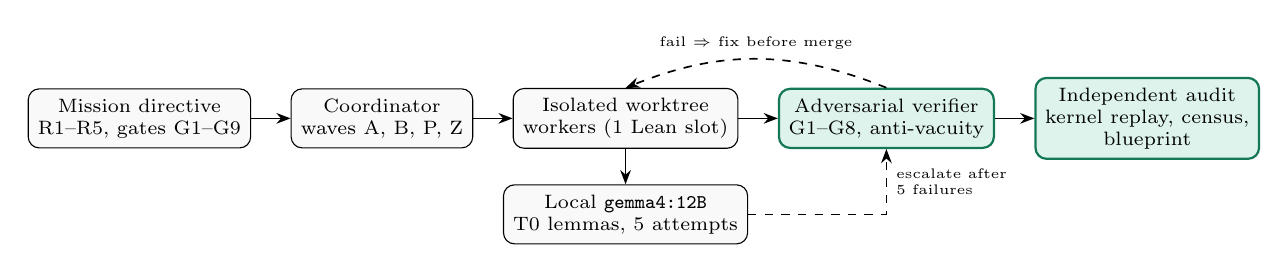
\begin{tikzpicture}[node distance=4.5mm and 5.0mm, every node/.style={font=\scriptsize},
  box/.style={draw,rounded corners,align=center,inner sep=3.5pt,minimum height=7.5mm,fill=gray!5},
  gate/.style={draw,rounded corners,align=center,inner sep=3.5pt,minimum height=7.5mm,fill=bpgreen!15,
               draw=bpgreen!70!black,thick},
  arr/.style={-{Stealth[length=1.8mm]},semithick}]
\node[box] (dir) {Mission directive\\R1--R5, gates G1--G9};
\node[box,right=of dir] (coord) {Coordinator\\waves A, B, P, Z};
\node[box,right=of coord] (work) {Isolated worktree\\workers (1 Lean slot)};
\node[box,below=of work] (gemma) {Local \code{gemma4:12B}\\T0 lemmas, 5 attempts};
\node[gate,right=of work] (ver) {Adversarial verifier\\G1--G8, anti-vacuity};
\node[gate,right=of ver] (aud) {Independent audit\\kernel replay, census,\\blueprint};
\draw[arr] (dir)--(coord);
\draw[arr] (coord)--(work);
\draw[arr] (work)--(ver);
\draw[arr] (ver)--(aud);
\draw[arr] (work)--(gemma);
\draw[arr,dashed] (gemma.east) -| node[pos=0.75,right,font=\tiny,align=left]{escalate after\\5 failures} (ver.south);
\draw[arr,dashed] (ver.north) to[bend right=22] node[above,font=\tiny]{fail $\Rightarrow$ fix before merge} (work.north);
\end{tikzpicture}%
}
\caption{Engineering and verification pipeline. Workers and verifiers used frontier models; routine
lemmas went first to a local model with compiler-in-the-loop checking.}
\label{fig:pipeline}
\end{figure}

\paragraph{1. Milestones with exclusive file ownership.}
The CMPP mission ran in waves (digit geometry and primitives; relocation and realization; Bennett,
universal machine and simulator; Poisson--Hamiltonian realization; final assembly). Each milestone
was developed in an isolated worktree and merged only after an independent verifier re-ran the
build, axiom audit, statement-freeze diff, wiring audit and refutation tests.

\paragraph{2. Local-model provenance.}
Lemmas tagged \code{T0} were attempted first by a local \code{gemma4:12B} model with Lean checking.
The ledger (independently re-read) records 646 calls; on 146 \code{T0} lemmas, pass@1 was
$40/146$ (27.4\%) and pass@5 $71/146$ (48.6\%); harder tiers stayed with frontier models.

\paragraph{3. This audit.}
The audit avoided the repository's own scripts for its core claims: kernel replay with the
toolchain's \code{leanchecker}, a fresh axiom census, binder and instance checks, a dependency
integrity check, and a blueprint written from the Lean sources and the paper, whose \NLeanDecls{}
declarations were re-checked for axioms.

\begin{thebibliography}{99}\footnotesize\sloppy
\setlength{\itemsep}{1pt}
\bibitem{CMPP21} R.~Cardona, E.~Miranda, D.~Peralta-Salas, F.~Presas, Constructing Turing complete
  Euler flows in dimension 3, \emph{PNAS} \textbf{118} (2021).
\bibitem{Lean4} L.~de Moura, S.~Ullrich, The Lean~4 theorem prover and programming language,
  \emph{Proc.\ CADE-28}, LNCS \textbf{12699} (2021), 625--635.
\bibitem{mathlib} The mathlib Community, The Lean mathematical library, \emph{Proc.\ CPP 2020}, 367--381.
\bibitem{TaoPFR} T.~Tao, Formalizing the proof of PFR in Lean4 using Blueprint: a short tour, 2023.
\end{thebibliography}

\newpage
\appendix
\section{Blueprint Dependency Graph}\label{app:graph}

\begin{center}
\vspace{0.5em}
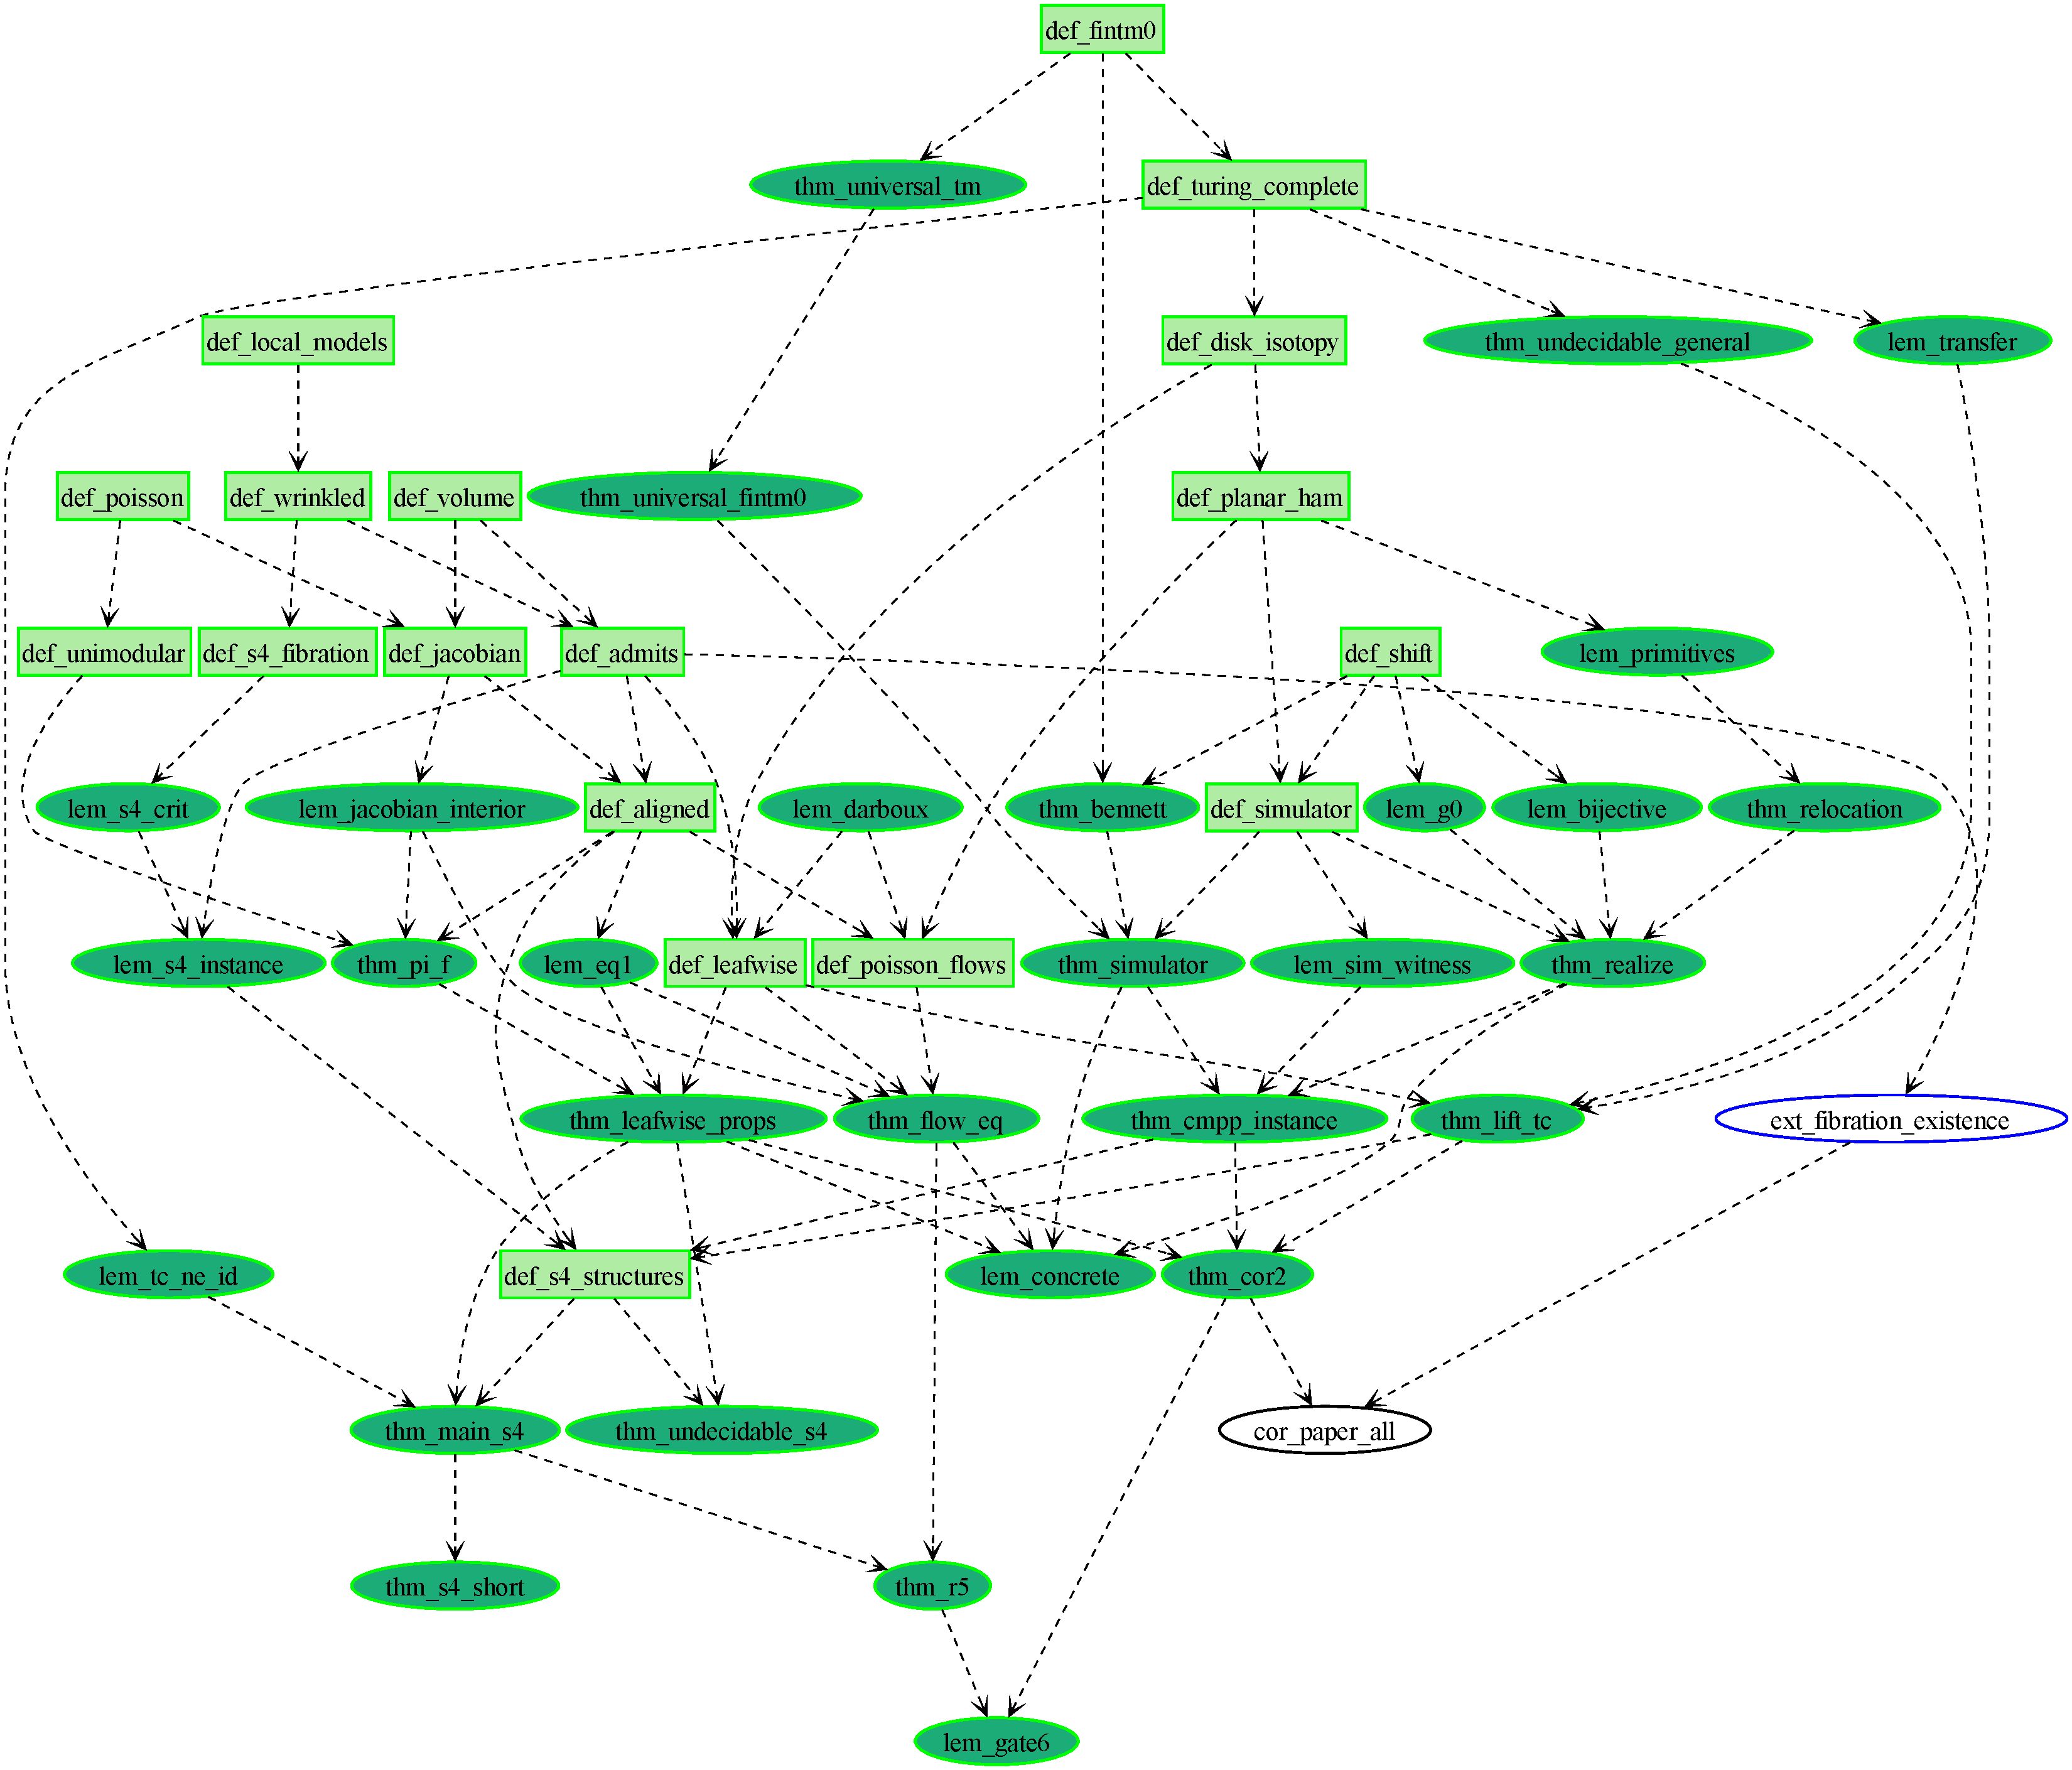
\includegraphics[width=\linewidth,height=0.80\textheight,keepaspectratio]{blueprint_dep_graph.pdf}
\end{center}
\vspace{0.5em}
\noindent\footnotesize\sloppy
\textbf{Figure A.1: \code{leanblueprint} dependency graph (portrait).}
Generated from \code{blueprint/src/content.tex} by \code{build\_dep\_graph.py}; interactive version
at \code{blueprint/web/dep\_graph\_document.html}. Arrows point from a node to the nodes that use it.
\textbf{Rectangles (\NDefNodes{}, \code{\#B0ECA3}):} formalized definitions.
\textbf{Filled ellipses (\NProvedNodes{}, \code{\#1CAC78}):} theorems proved in Lean with
\code{0 sorryAx} and standard axioms across their dependency closure.
\textbf{Unfilled ellipses (\NOpenNodes{}):} \code{ext\_fibration\_existence} and
\code{cor\_paper\_all}, the paper's Corollary~2 for every closed oriented $4$-manifold, not formalized
(finding F1).\par

\end{document}
